\subsection{Following Links Between Categories}
\label{sec:following_links_between_categories}
Finding the full paths for each Wikipedia article can be done when the representation of the structure is ready. Each path can be found by following the links between categories until an article is reached, and the category links visited form an article path. 

\begin{figure}[h]
\centering
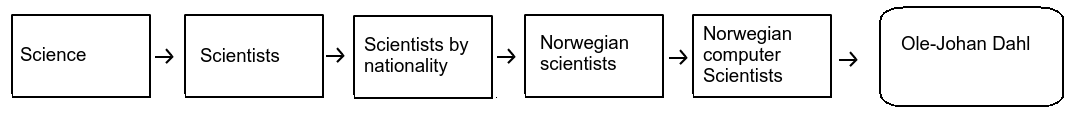
\includegraphics[width=\textwidth]{Chapters/Implementation/example_path}
\caption[Example of an article path]{Example of one of the article paths of the article \emph{Ole-Johan Dahl}. The rectangles are categories and the rectangle with rounded corners is the article. }
\label{fig:examplepath}
\end{figure}

\subsubsection{Issues with finding the full path}
The structure of Wikipedia is not represented as a tree, but as a graph. This means that there might be loops within the graph. A loop within the graph means that a category already visited in the search of a path can be reached again. Figure \ref{fig:exampleloop} shows an example  of a path which contains a loop.

% 177820/907585/173722/572284/531983/173722
% people/fictional characters/fictional characters by species/fictional life forms/legendary creatures in popular culture/fictional characters by species
\begin{figure}[h]
\centering
\begin{lstlisting}
people/fictional characters/fictional characters by species/fictional life forms/legendary creatures in popular culture/fictional characters by species
\end{lstlisting}
\caption{Example of a loop found in a path.}
\label{fig:exampleloop}
\end{figure}


This could lead to a problem if the program keeps going in loop, and does not reach an article. A solution to this problem is to keep track on categories already visited and only follow links to categories not yet visited in the path. 
%This might mean that the path to the category is not the best one, but 

Another issue is to decide the start point for the paths, in other words decide the start category. Wikipedia contains some natural categories that are better to use as start categories. These categories are very general and have links to some of the major categories within different fields, thus, able to reach most other categories in the Wikipedia category structure. The category \emph{Main Topic Classifiers} was chosen for this task, because it has 22 subcategories within various fields and  where all of them have their own subcategories (see figure \ref{fig:mainclassifiers})\cite{wiki:specialtree}.

\begin{figure}[h]
\begin{center}
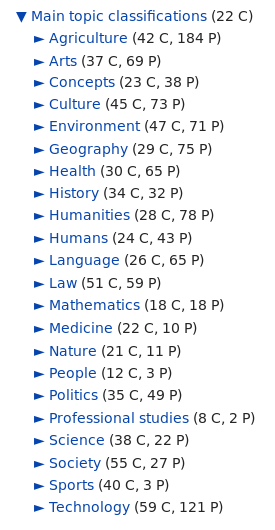
\includegraphics[width=0.4\textwidth]{Chapters/Implementation/Maintopicclassifiers.png}
\end{center}
\caption[Subcategories of \emph{Main Topic Classifiers}]{Illustrates the first subcategories of the chosen start category \emph{Main Topic Classifiers}. \emph{C} corresponds to the number of a category's subcategories and \emph{P} corresponds to its number of pages. The figure is provided by Wikipedia's Category Tree.} % TODO: \cite{wiki:specialtree}.}
\vspace{-20pt}
\label{fig:mainclassifiers}
\end{figure}

%The category \emph{Main Topic Classifiers} has a large variety in its subcategories which makes it possible to reach categories within many topics. 

